\newpage
\section{Decider for ``Translated Cyclers''}\label{sec:translated-cyclers}

\begin{figure}[h!]
  \centering
  % 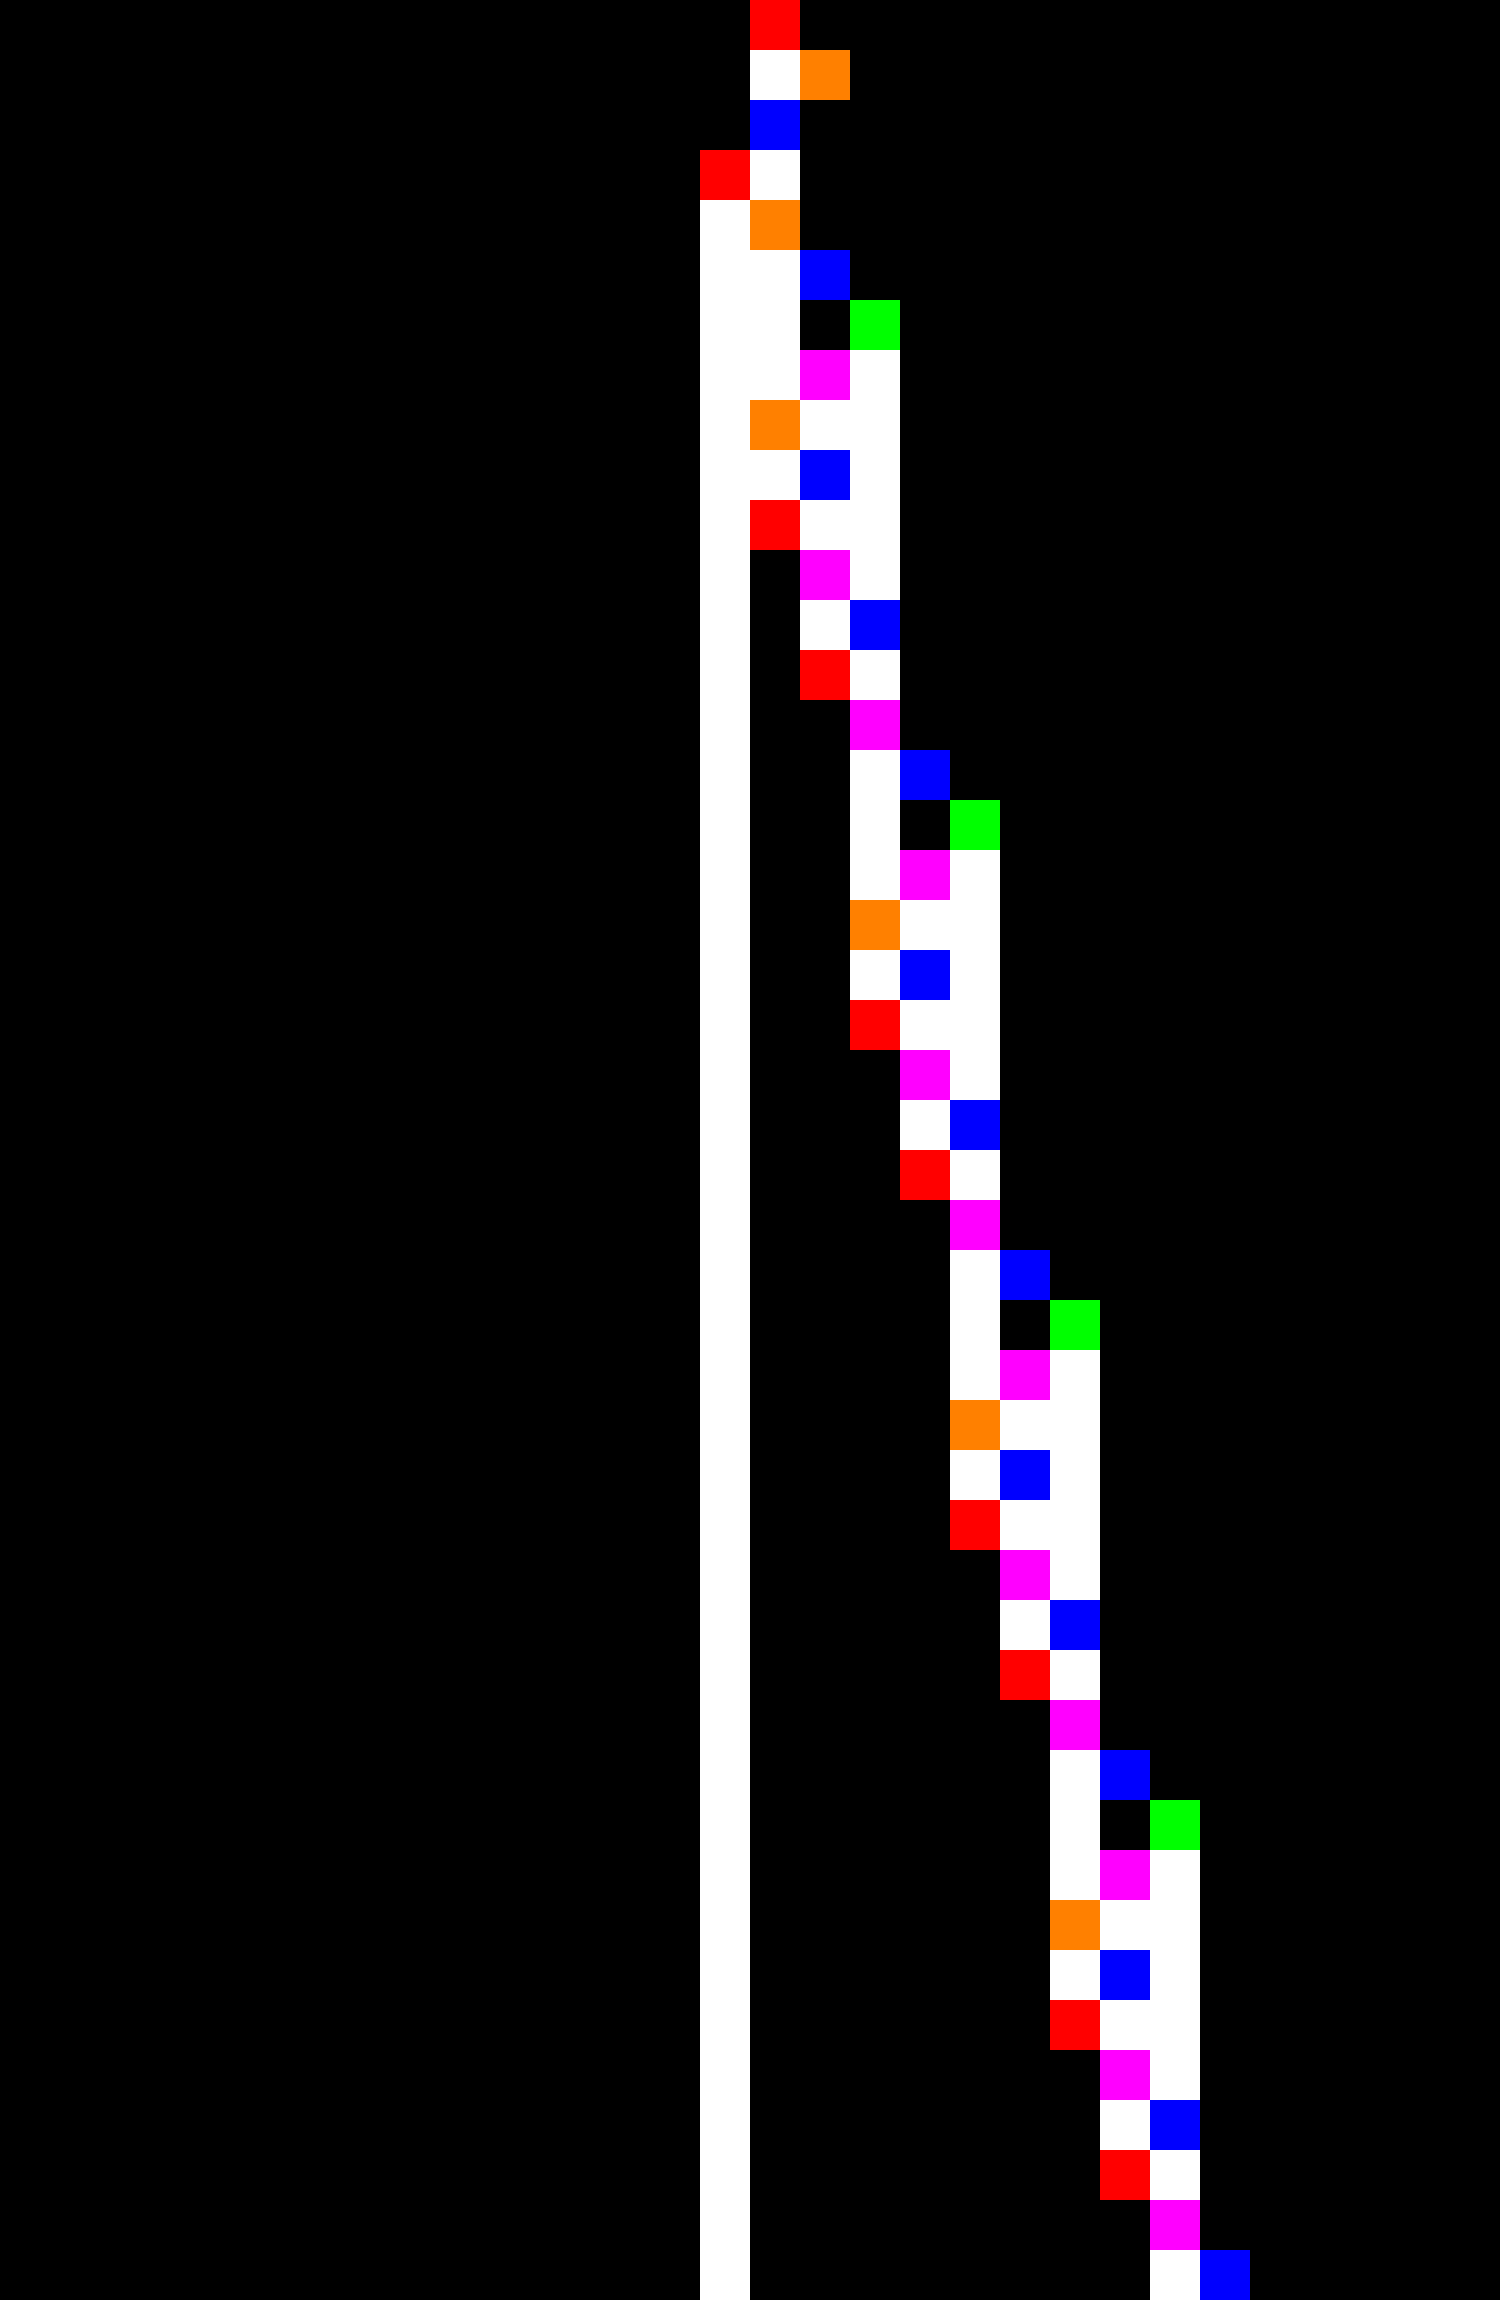
\includegraphics[width=0.5\textwidth]{space-time-diagrams/translated_cycler_44394115.pdf}
  % \hspace{2ex}
  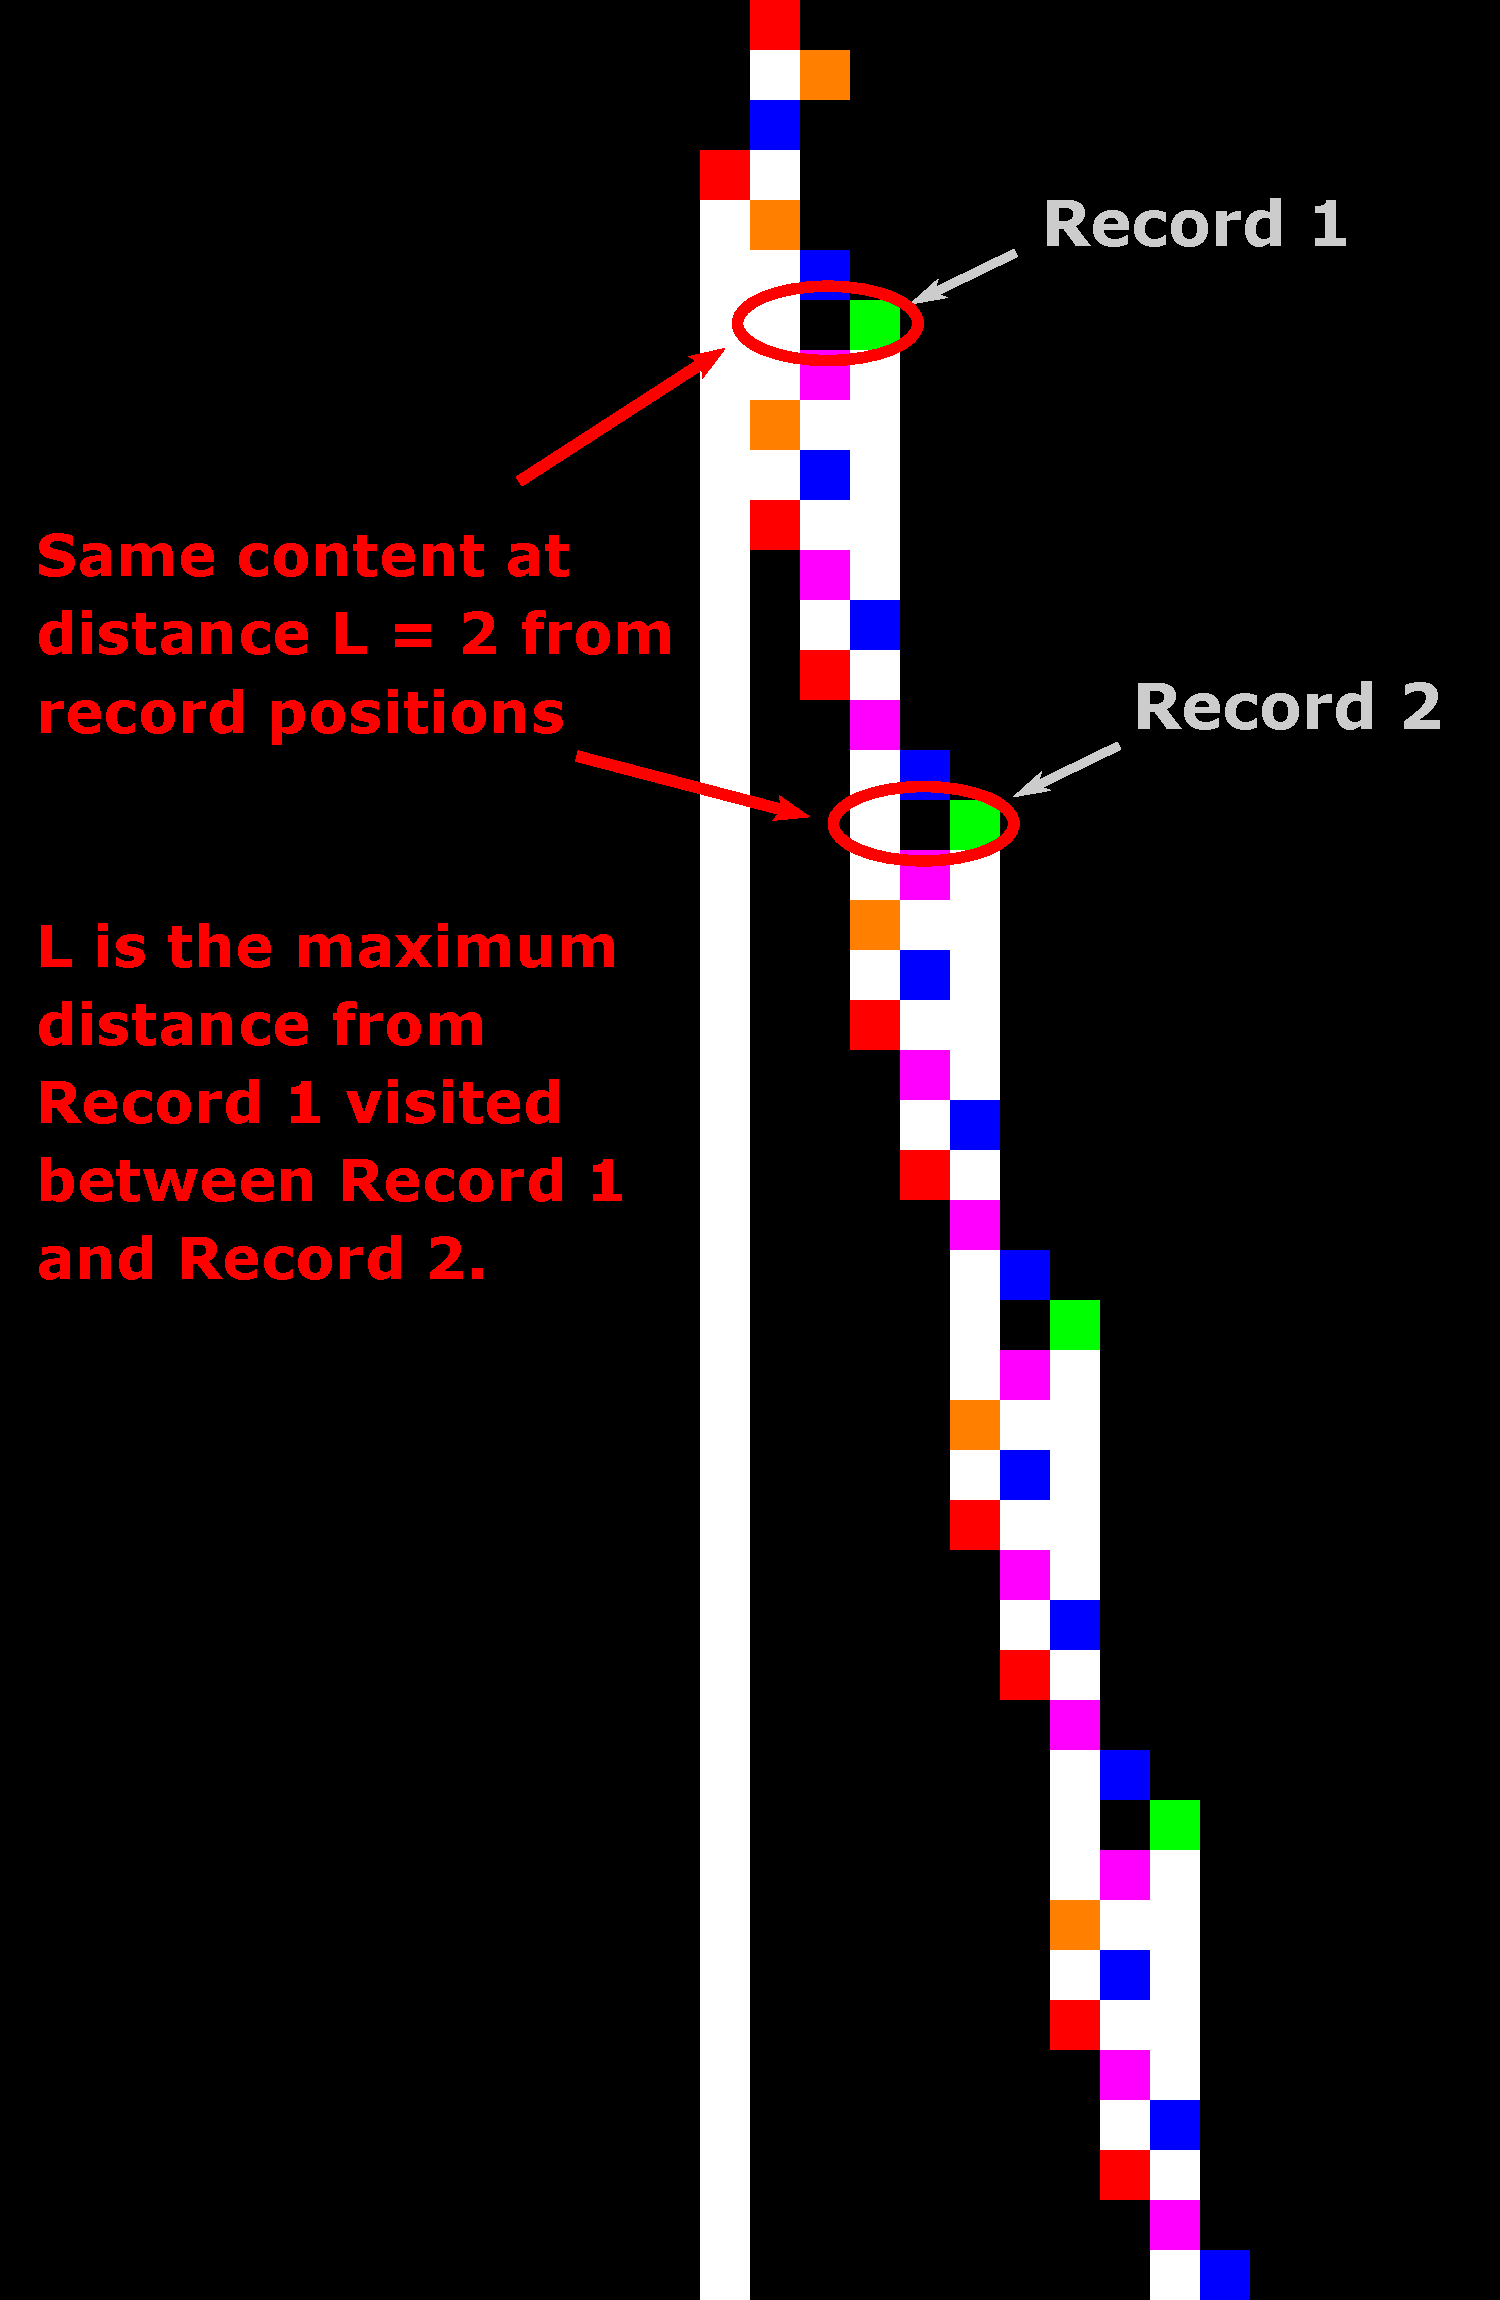
\includegraphics[width=0.54\textwidth]{space-time-diagrams/translated_cycler_44394115_annotated.pdf}

  \caption{Example ``Translated Cycler'': bbchallenge's machine \#44,394,115, see \url{https://bbchallenge.org/44394115}. The same bounded pattern is being translated to the right for ever. The text annotations illustrate the main idea recognising ``Translated Cyclers'': find two configurations that break a record (i.e. visit a memory cell that was never visited before) in the same state (here state \textcolor{colorD}{D}) such that the content of the memory tape at distance L from the record positions is the same in both record configurations. Distance L is defined as being the maximum distance to record position 1 that was visited between the configuration of record 1 and record 2.}\label{fig:translated-cyclers}
  \end{figure}
  
  The goal of this decider is to recognise Turing machines that translate a bounded pattern for ever. They are close to Cyclers (Section~\ref{sec:cyclers}) in the sense that they are only repeating a pattern but there is added complexity as they are able to translate the pattern in space at the same time, hence the decider for Cyclers cannot directly apply here.
  
  \begin{example}\normalfont
  Figure~\ref{fig:translated-cyclers} gives the space-time diagrams of 
  \end{example}